\documentclass[11pt,preprint]{aastex}

\begin{document}
\def\simlt{\lower.5ex\hbox{$\; \buildrel < \over \sim \;$}}
\def\simgt{\lower.5ex\hbox{$\; \buildrel > \over \sim \;$}}

\title {EXPLORING DIGITAL SAMPLING, FOURIER TRANSFORMS, and the DSB MIXER}

\tableofcontents

	The purpose of this lab is to experimentally investigate digital
sampling, digital Fourier transforms, and mixers. Mixers are the basis
of heterodyne spectroscopy. Heterodyne spectroscopy, in turn, is what you
use every day that you listen to a radio, use a cell phone, or watch
TV---or do radio astronomy. You will be performing several experiments,
analyzing the data and generating a number of
different data files. You will need to keep careful notes in your {\bf
lab notebook}! Or, pay the penalty, and forget what you did, do things
twice, and be completely disorganized. Your choice!

\section{GOALS}

\begin{itemize}

\item Learn how to sample electronic signals---here, one or more sine
  waves---digitally using our computers.

\item Become acquainted with the basic law of sampling: the Nyquist
  criterion.

\item Learn how to use Digital Fourier Transforms (or Discrete Fourier
  Transform; DFT) to determine the
  frequency spectrum of a signal.

\item Learn about the Fast Fourier Transform (FFT) as a particular, and
  particularly fast, implementation of the DFT.

\item Learn the basics of mixing for frequency conversion (that's
  the {\it heterodyne} technique) and for measuring phase.

\item Get started with our programming language, IDL, using it for the
  mathematical analysis, signal processing, and making nice plots.

\item Learn enough Latex to write up your results in a formal lab report,
  including nice plots and graphs.

\end{itemize}

\section{SCHEDULE}

There's a lot to do in this lab! If you don't understand the Nyquist criterion
by the end of the first week, you're behind. Here's how it should be:
\begin{enumerate}

\item {\it The First Week, 19 Jan to 25 Jan:} Finish \S \ref{nyquist},
  \S \ref{pwrspectrum}, \S \ref{leakage} below. Be prepared to show your
  results to the class, making real-time plots in IDL.

\item {\it The Second Week, 26 Jan to 1 Feb:} Finish \S \ref {upperlowerdsb} and \S
  \ref{phasedetector} below. Again, be prepared to show your results to
  the class.

\item {\it The Third Week, 2 Feb to 8 Feb:} Write your formal report!
  It should follow the standard format, consisting of an introduction,
  discussion of experimental activities and results, description of the
  analysis technique, presentation of analysis results, and
  discussion/interpretation. With all this, you should hand in a
  reasonable number of plots together with commentary to illustrate your
  work, your thought processes, and your conclusions.

\end{enumerate}

\section{\ NYQUIST SAMPLING AND ALIASING: A SINGLE SINE WAVE (First Week)} \label{nyquist}

	Here we explore the all-important realms of the Nyquist
criterion and aliasing in digital sampling.  Clearly, if you sample too
slowly the signal won't be well-reproduced.  But if you sample really
fast, then you generate large data files that take a long time to
process.  Just how slowly can you sample the signal without completely
losing its basic properties (such as, for example, the fact that it
oscillates with frequency $\nu_{sig}$)?

The fundamental parameter here is the ratio of sampling frequency
$\nu_{smpl}$ to signal frequency $\nu_{sig}$. With our equipment we can set
$\nu_{smpl}$ to only selected, quantized values. However, we can set
$\nu_{sig}$ with almost arbitrarily high precision. So to explore these
issues we will pick a sampling frequency $\nu_{smpl}$ and take data at
several signal frequencies $\nu_{sig}$.  Be sure to use a coax T so that
you can look at the sampled signal on the oscilloscope.  Set the
peak-to-peak voltage appropriately so that it doesn't saturate the
Analog-to-Digital Converter (known as the ADC).

\subsection{Your First Digital Sampling}

	We want to explore sampling rate issues, so to that end
we will begin by\dots \begin{enumerate}

	\item Pick a convenient sampling frequency $\nu_{smpl}$.  

	\item Set the synthesizer to frequency $\nu_{sig} = (0.1, 0.2,
	  0.3, \dots, 0.9) \nu_{smpl}$ and take data. 

\end{enumerate}

\noindent Take $N$ contiguous samples with $N$ an integral power of 2, say
$N=256$.  Throughout the datataking, you should always be
monitoring the signal with the oscilloscope. These are sine waves, so
it's easy to measure the period by looking at the oscilloscope; each
time you digitally sample the signal, you should write down the period
(maybe in your {\it lab notebook?}).  

For each dataset, use IDL to plot the digitally sampled waveform versus
time.  In particular, make the digital plot informative, meaning that
you can clearly see the signal shape; if necessary, plot only a part of
the data so you can clearly see the signal shape (e.g., a few cycles of
the sine wave); compare this with the oscilloscope trace.  Also, for all
the datasets derive and plot the Fourier power spectrum.  Make sure that
you {\it label the axes} with proper values of time and frequency---and
choose convenient units, such as microsec and megaHz, to avoid huge and
tiny numbers.  In deriving the Fourier spectra, use our homegrown DFT
procedure (see \S \ref{pwrspectrum} below).

Now, {\it look at both sets of these plots} and note any funny business.
Think about your results and draw your own conclusion: just what is the
minimum sampling rate that you can get away with? (That's {\it Nyquist's
  criterion)}. 

\subsection{Let's Go to Extremes\dots}

By now you might have an idea of what's going on. Test yourself:
try the following two experiments. But before analyzing the
results, {\it predict} to yourself what they will look like. How? Use
good old-fashioned paper and pencil to make some diagrams. If you can
successfully predict the following, then you {\it really} understand
the Nyquist criterion! So here we go: \begin{enumerate}

\item Repeat the above for $\nu_{sig} = \nu_{smpl}$. 
\item Now make $\nu_{sig} \over \nu_{smpl}$ {\it really {\Large large!}}
	    In other words, {\it blatantly violate} Nyquist's criterion!
	    Our oscillators won't run faster than 30 MHz, so to
	    accomplish this you'll have to use not only a large
	    $\nu_{sig}$ but also change $\nu_{smpl}$ to be very
	    slow. Use as large as a ratio as you can, but make sure that
	    the ratio is {\it not} an integral or half-integral number. Take lots of
	    samples. Look at the sampled waveform.  What do you get?
	    Why?
\end{enumerate}

\subsection{For your Lab Report}

\noindent In your report, select a well-considered set of plots to
illustrate what you've learned, and compose a well-written commentary
that convinces me that you really understand what's going on. Also
clearly state what you have concluded regarding Nyquist's criterion. 

	With your plots, you can save paper by fitting multiple plots on a page
by using IDL's \verb$!p.multi$ system variable; for example, if you
wanted 4 plots running vertically down the page you'd set
\verb$!p.multi=[0,1,4]$; if you wanted two columns of 4 plots down the
page, you'd set {\tt !p.multi=[0,2,4]}.  To get back to one plot per page, set
\verb$!p.multi=0$. 

\section{ ON USING DFT AND FFT TO CALCULATE A POWER SPECTRUM (First Week)} 
\label{pwrspectrum}
 
\subsection{The Analytic Fourier Transform}

        The input to the Fourier transform is voltage versus time, say
$E(t)$; the output is voltage versus frequency, say $E(\nu)$.  The Fourier
transform is the integral
 
\begin{equation}
E(\nu) = {1 \over T} \int_{-T/2}^{T/2} E(t) e^{2 \pi j \nu t} dt \ .
\end{equation}
 
\noindent The input voltage is real; it is multiplied by the complex
exponential and integrated, so the output is complex. Of particular
importance is that he Fourier Transform is {\it invertable}: you can go
from the time to the frequency domain, and from the frequency domain you can
get back to the time domain using the inverse transform

\begin{equation}
E(t) = {1 \over F} \int_{-F/2}^{F/2} E(\nu) e^{-2 \pi j \nu t} dt \ .
\end{equation}
 
\noindent {\it Note:} If you're paying attention, you would wonder how
$F$ and $T$ are defined above. In the proper analytic formulation, they
are both infinity. We emphasize their boundedness here because, in
practice, i.e.\ when you do numerical calculations, neither can be
infinity!

\subsection{The Discrete Fourier Transform (DFT)} \label{dft}

Our voltage versus time is not continuous, but rather it is discrete
samples. With the digital transform, the integral becomes a sum. In
this sum, you need to specify: \begin{enumerate}

\item The set of sample times. I {\it strongly} suggest: \begin
 {enumerate}
\item  Using $N$ samples, where $N$ is even (and even better: a power of 2).

\item Use the center
  channel as the zero point. With $N$ even, there is no center channel,
  so make the times run from ${-N \over 2}/
  \nu_{smpl}$ to $({N \over 2} -1)/ \nu_{smpl}$.
\end{enumerate}

\item The output is a function of frequency, so you have to specify the
  frequencies for which you want the output $E(\nu)$. I {\it strongly}
  suggest that, {\it at first}, you calculate the the output for $N$
  frequencies running from $-{\nu_{smpl} \over 2}$ to $+{\nu_{smpl}
  \over 2} \left( 1 - {2 \over N} \right)$. This makes the frequency
  increment equal to  $\Delta \nu = \nu_{smpl}/N$. Thus, you
  calculate a {\it voltage} spectrum running from $-{\nu_{smpl} \over
  2}$ to about ${\nu_{smpl} \over 2}$ using our in-house DFT procedure. To
  find out how to use DFT, use the {\tt doc\_library} or {\tt doc}
  function; in IDL, type:\ \ {\tt doc, 'dft'}.

Later on, if you are intellectually daring and curious, try doubling or
tripling the frequency range, keeping the separation $\Delta \nu$ the
same (i.e., by increasing the number of output frequencies to $2N$ or $3N$).

\end{enumerate}

        We are interested in the output {\it power spectrum}, say
$P(\nu)$.  Power is voltage squared.  For complex quantities, the squaring
operation means we want the sum of the squares of the real and imaginary
parts.  We obtain this by multiplying the voltage by its complex
conjugate,
 
\begin{equation}
P(\nu) = E(\nu) E(\nu)^* \ .
\end{equation}
 
\noindent In IDL, there are two ways to get this product.  One is to use
the \verb$conj$ function, i.e.\ {\tt PF = EF * conj(EF)}.  Should the
imaginary part of \verb$PF$ be zero? (answer: yes! Why is this?) Is it?
(answer: no! Why not?) To get rid of this annoying and extraneous
imaginary part, you can use the \verb$float$ function: 
\verb$PF = float(PF)$. 
 
The other (more convenient and suggested) way is to square the length of
the complex vector, i.e.\ \verb$PF = (abs(EF))^2$. The result is
automatically real.

\subsection{OPTIONAL: The Fast Fourier Transform (FFT)} \label{fft}

Above in \S \ref{dft}, you had $N$ time samples and evaluated the DFT
for $N$ well-chosen frequencies. These were ``well-chosen'' because for
these particular values of frequency---and {\it only} these particular
values---you can get back to the time domain by using the inverse
transform (in IDL using {\tt dft}, you accomplish this by setting the
{\tt inverse} keyword). {\it If you have the time and energy}, try this
and make it work!

It so happens that, for these particular combinations of frequency and
time, there is a very fast algorithmic implementation called the {\it
  Fast Fourier Transform}, the FFT. What do we mean by ``Fast''? Well,
normally when you do a DFT, you have $N$ input numbers and $N$ output
numbers and the number of calculations $\propto N^2$. When $N$ gets large,
this takes a long time to calculate! For the FFT, on the contrary, the
number of cdalculations $\propto N {\rm ln}_2(N)$, and this makes it
possible to do large-$N$ transforms. 

{\it If you have the time and energy}, try IDL's FFT and compare it to
your DFT calculation above. The FFT output is ordered in what you might
think is a funny and awkward way; however, it's really {\it not} awkward
for most applications. See our ``DFT's with DFT's'' handout for details.

\section{ LEAKAGE POWER AND FREQUENCY RESOLUTION (First Week)} \label{leakage}

\subsection{Leakage Power}

Above, you calculated a power spectrum for each input signal at $N$
distinct frequencies separated by $\Delta \nu = \nu_{smpl}/N$. In each,
you found a spike corresponding to the input signal's frequency. Here,
focus on just one of the properly-sampled signals $\nu_{sig}$. Calculate
the power spectrum for many more than $N$ output frequencies over the
Nyquist range $\left[-{\nu_{smpl} \over 2} \ {\rm to}\ +{\nu_{smpl}
\over 2} \left( 1 - {2 \over N} \right)\right]$; i.e., make the
frequency increment much smaller than $\Delta \nu = \nu_{smpl}/N$.
Making the output frequencies closer together gives a more nearly
continuous frequency covereage in the plot of the output spectrum.  Turn
up the vertical scale a lot to see if there is any nonzero power at
frequencies other than $\nu_{sig}$.  You {\it do} see such power! This
is {\it Spectral Leakage}. It affects all power spectra calculated using
Fourier techniques. 

Can you understand what's going on from a mathematical viewpoint?

\subsection{Frequency Resolution}

If you had two sharp spectral lines, how closely spaced in frequency
could they be and still resolve them? Roughly, this is just the apparent
width of the line when plotted against frequency. Look at the width of
the line for your plot of \S \ref{leakage} above. Compare this width to
$1 \over T$, where $T$ is the total time span over which the samples
were taken. If you have the inclination, try taking other time series
with varying number of samples (and thus, varying $T$) and confirm any
relationship between line width (that is, frequency resolution) and
$T$.

Can you understand this from a mathematical viewpoint?

\section{ BASIC DOUBLE SIDEBAND (DSB) MIXER OPERATION: UPPER AND LOWER
  SIDEBANDS (Second Week)}
\label{upperlowerdsb}

        For this, use two SRS synthesizer oscillators as inputs to a
mixer to explore the spectra and waveforms in the DSB mixing process.
The SRS synthesizers work up to 30 MHz.  Assign one of the SRS
synthesizers to be your ``local oscillator'' ({\it lo}) with frequency
$\nu_{lo}$, and the other your ``signal'' with frequencies $\nu_{sig} =
\nu_{lo} \pm \delta \nu$.  Here, you choose the frequency difference
$\delta \nu$ and you set the two synthesizers, one to the lo
frequency and the other to the signal frequency. There are two cases for
the signal freqquency, $\nu_{sig} = \nu_{lo} + \delta \nu$ and
$\nu_{sig} = \nu_{lo} - \delta \nu$.  Make $\delta \nu$ somewhat small
compared to $\nu_{lo}$, maybe $5\%$ of $\nu_{lo}$.  For the input power
level, a good choice is 0 dbm\footnote{What does this ``dbm'' mean? It's
the power relative to 1 milliwatt, expressed in decibels (db). For our
system the cable impedence is 50 ohms; what's the rms voltage for a
signal with power level 0 dbm?} for both synthesizers.

        We will want to digitally sample the mixer output and explore
both the sum and difference frequencies. As you learned in the Fourier
lab, there are extremely important issues regarding sampling rate. The
most basic is the Nyquist criterion. For this lab, we also want enough
samples per period to give you a reasonable facsimile of the sine wave
when you plot it; from this standpoint, it's not unreasonable to sample
at twice Nyquist, or even faster.  Another issue is the {\it number of
points} you sample, which must be large enough to give you at least a
few periods of the slowest sine wave.

        From what you know about mixers, what is the fastest sine wave
in the output? This, combined with our above comment and the upper limit
on our sampling frequency (20 MHz for single channel, 10 MHz for dual
channel), would determine the upper limit on $\nu_{lo}$.

\subsection{The Mixer}

Combine the two signals, $\nu_{lo}$ and $\nu_{sig}$, in a mixer for the
two values of $\nu_{sig}$.  For the mixer use a Mini-Circuits
ZAD-1, which has three BNC connectors (three {\it ports}) and works well
at these frequencies.  The ZAD-1, like nearly all mixers, has its ports
labeled ``R'' (the ``RF'' or ``signal''); ``L'' (the ``local
oscillator''); and ``X'' (the ``mixing product'') or ``I'' (the
``intermediate frequency'').  However, as we explain below, these labels
are misnomers.  They are based on the usual use for a mixer, which is to
take two high frequency signals as the inputs to the R and L ports and
produce a low frequency difference frequency as the output at the I
port.

        The ZAD-1 is a balanced mixer, so the ``R'' and ``L`` ports are
identical, and in particular will not couple to DC or very low
frequencies.  In contrast, the ``I'' port is coupled differently and
will handle voltages all the way down to, and including, DC.  The mixing
process functions no matter which two ports are used as inputs.  For
example, if you are using a mixer to modulate a high frequency (say, a
few MHz) with a low frequency (say, a few kHz), you should use the ``I''
port for the low frequency and either of the other two for the high
frequency; take the output from the third port.

We will want to look at the output, which consists of both the sum
and difference frequencies, so choose the ports appropriately. Digitally
sample the mixer output for both cases ($\nu_{sig} = \nu_{lo} \pm \delta
\nu$).

\subsection{For Your Lab Report} \label{digsamp}

        For the two cases, plot the power spectra versus
frequency. Explain why the plots look the way they do. In your
explanation include the terms ``upper sideband'' and ``lower sideband''.

For one of the cases, plot the waveform.  Does it look like the
oscilloscope trace? Also, take the Fourier transform (not the power
spectrum) of the waveform and remove the sum frequency component by
zeroing both the real and imaginary portions (this is ``Fourier
filtering'').  Recreate the signal from the filtered transform by taking
the inverse transform; see \S \ref{fourierfilter} to see how this is
done. Plot the filtered signal versus time.  Explain what you see.

\subsection {On  Fourier Filtering} \label{fourierfilter}

When you use DFT to go from the time to the frequency domain, you
specify the times and the sampled voltages as input and calculate the
output for a well-chosen set of frequencies.  These times and
frequencies should be symmetric around zero, as we strongly suggested above in \S
\ref{pwrspectrum}.  To filter out the high-frequency mixed signal, you
have to zero both the real and imaginary high-frequency components,
and you must zero both the negative and positive frequencies. In
frequency space, these zeroed values {\it must} be symmetric.

To go back from the frequency domain to the time domain, use the 
  filtered frequency Fourier components (which are complex) and their associated frequencies
  as {\it inputs} and calculate the output for the {\it original times}.
  You should also set the {\tt inverse} keyword in DFT, which keeps the
  amplitude scale correct (check the documentation for DFT using {\tt
  doc\_library} or {\tt doc}). The output will be a time series, and because you've
  eliminated the sum frequency component, the only thing that remains
  should be the difference frequency component.

One more thing. The output of the inverse transform had better be
real---after all, your original input was real! You'd better check this!
If it isn't real, then either (1) you didn't treat the negative and positive
frequencies symmetrically when you zeroed the signal, or (2) you didn't
use our suggested input times and output frequencies. If you're having
trouble, check your basic technique by doing the inverse transform on
the non-filtered Fourier components; you should recover the original
time samples.

\section{DSB MIXER AS A PHASE DETECTOR (Second Week)} \label{phasedetector}

        Use a mixer as a phase detector by setting the two synthesizers
to the same frequency, i.e.\ setting $\delta \nu = 0$.  Look at the
mixer output on the oscilloscope.  Vary the phase of one of the
synthesizers.  What happens to the mixer output as shown on the
oscilloscope trace? What's going on here?

Now measure the mixer output with the HP rack-mounted digital meter in
its d.c.\ mode, reading it with the computer.  The d.c.\ mode is akin to
a low pass filter because the sum frequency, which is a fast sine
wave, contains no d.c.  Generate a file that contains both the phase and
the d.c.\ voltage and plot (to hand in!) the result.  If you're clever,
you can write an IDL script to take the data automatically.  How does
this correspond to the interferometer fringe?

        Now displace one of the synthesizer frequencies by some small
amount---say, 1 Hz. What happens to the output? This should remind you
of the interferometer fringe\dots

        {\it For your lab report}, hand in appropriate plots and discussion.


\section {SOME COMMENTARY}

Mixers are important because they allow us to shift the
frequency of the whole input spectrum by a uniform amount.  They do this
by multiplying the input signal by the ``local oscillator'' (l.o.) with
frequency $\nu_{lo}$; this shifts the frequencies by $\nu_{lo}$.  In radio
reception, this is very important because nearly always our {\it
detectors} work best in a fixed frequency range, but our {\it signals}
come in at many different frequencies.  For example, for an AM station
playing rock music, the ultimate detector is our ear, which works only
at audio frequencies; however, the AM stations transmit at much higher
frequency, nearly 1 MHz.  A mixer is used to shift the frequencies of
the AM station down to the audio region.  Such receivers are called {\it
heterodyne} receivers, and this principle is used universally not only
in consumer radios, TV's, and cellphones but also in many other
applications including radio astronomy.

        For example, later in the course we have the 21-cm line at
1420.4 MHz and use an l.o.\ at 1270.4 MHz, the difference frequency is
150.0 MHz and the sum frequency is 2690.8 MHz.  We use a low-pass filter
to obliterate the sum frequency, so we are left with a replica of the
21-cm line that is centered at 150.0 MHz instead of 1420.4 MHz.  If the
Doppler shift from the Earth's orbit (for example) shifts the 21-cm line
from 1420.4 to 1420.0 MHz, we change the l.o.\ frequency to 1270.0 MHz
so that the line remains centered at 150 MHz.  In this way, our
spectrometer can always work at the same frequency, 150 MHz.

        Mixers are crucially central to the important radioastronomical
technique called interferometry.  In this technique, two
widely-separated telescopes point at the same source.  Usually, the
radio source is further from one telescope than the other, which
produces a phase difference $\phi$ between the signals from the two
dishes.  The two received signals from the source are combined in a
mixer, which produces a d.c.\ voltage that is proportional to $\sin
\phi$. The phase difference changes with time, which leads to d.c.\
voltage proportional to $\sin 2\pi f_{fringe}t$, where $f_{fringe}$ is
the local fringe fringe frequency and is equal to $d\phi \over dt$.  You
can also think of of this sinusoidal phase resulting from the differing
velocities $\Delta v$ of the two telescopes with respect to the source,
with $f_{fringe}$ being the Doppler shift, equal to the observing
frequency times $\Delta v \over c$.

\section { SOME THEORY: THE ORDINARY DOUBLE SIDEBAND (DSB) MIXER}

        We now turn to the basic theory of the ordinary DSB mixer, which
is very straightforward.  An ideal mixer multiplies the two input
signals together; this multiplication makes the output signal have the
sum and difference frequencies.  Usually, one of these is eliminated by
using a filter.

        Suppose for simplicity that the mixer is ideal and that the two
input signals are the following: {\bf (1)} the ``local oscillator'' with
voltage equal to unity (for convenience) and frequency $\omega_0$; and
{\bf (2)} two ``signals'' with voltage $E_s$ and frequencies
$\omega_{s-} = (\omega_0 - |\delta \omega |)$ and $\omega_{s+} =
(\omega_0 + |\delta \omega |)$. We handle the two signal case
simultaneously by writing $\omega_{s \pm} = (\omega_0 \pm |\delta \omega
|)$.\footnote{In real life, e.g.\ a radio station, the ``signal'' is
speech or music with a broad range of $\delta f$. In astronomical life,
e.g.\ the 21-cm line, the ``signal'' is a Doppler broadened line, which
again has a broad range of $\delta f$. The system is linear, so signals
add without mutual interaction, so the discussion for a single $\delta
f$ also applies to these broad spectra.}

        The mixer outputs in the two cases are $MO_-$ and $MO_+$;
similarly, we write $MO_{\pm}$. $MO$ is the product of the signal and
l.o.~signals, and can be expressed in terms of the sum and difference
frequencies by the usual trig identity

\begin{mathletters}
\begin{equation}
MO_{\pm} = E_s \underbrace{\cos [\omega_{s \pm} t] \cos [\omega_0 t]
}_{product} =
        {E_s \over 2} (\underbrace {\cos [(\omega_{s\pm} - \omega_0)t
	]}_{diff} +
        \underbrace { \cos [(\omega_{s\pm} + \omega_0)t]) }_{sum}
\end{equation}

\noindent Replacing $\omega_{s\pm}$ by $\omega_0 \pm |\delta \omega|$,
we get


\begin{equation} \label{mopm}
MO_{\pm} = E_s \underbrace{\cos [(\omega_0 \pm |\delta \omega |)t]
\times
\cos [\omega_0 t]}_{product} = {E_s \over 2}
        (\underbrace{ \cos [\pm|\delta \omega | t]}_{diff} +
        \underbrace{ \cos[(2\omega_0 \pm |\delta \omega |) t]}_{sum} ) \
.
\end{equation}
\end{mathletters}

\noindent Thus, the signal frequency has been shifted to {\it two}
frequencies by an amount equal to the l.o.\ frequency:  downward in the
first term (to $\delta \omega $, the difference frequency) and upward
in the second term (to $2\omega_0 \pm |\delta \omega |$, the sum
frequency).  The output contains {\it both} the difference {\it and} the
sum frequency terms.

        Now we insert a low pass filter to eliminate the sum term. We do
this because we are observing at some very high frequency, say the 21-cm
line at 1.4 GHz, and need to convert to much lower frequencies where our
backend equipment works. (In the TV case it's the same: the signals are
at hundreds of MHz and the picture processing circuitry operates below
10 MHz). This low-pass filter removes the second term.

        So with the low-pass filter we drop the sum frequency term. This
leaves the following, in which we add the subscript $cos$ to indicate
that we began with the signal represented by a cosine:

\begin{mathletters} \label{baseband}
\begin{equation}
MO_{cos,\pm} = {E_s \over 2} \cos [\pm|\delta \omega | t] = {E_s \over
  2}
   \cos [|\delta \omega | t] \ .
\end{equation}

\noindent If we had begun by representing the signal with a sine instead
of a cosine (while retaining the cosine for the l.o.) we would have
obtained

\begin{equation}
MO_{sin,\pm} = {E_s \over 2} \sin [\pm|\delta \omega | t] = \pm {E_s
  \over 2}
   \sin [|\delta \omega | t] \ .
\end{equation}
\end{mathletters}

        Four things are important here: \begin{enumerate}

        \item {\it The two sidebands---the two different} input
frequencies ($[\omega_{s-}= \omega_0 - \delta \omega]$ and $[\omega_{s+}=
\omega_0 + \delta \omega]$)--- produce the {\it same
symmetric-around-zero pair of final output frequency $\pm |\delta
\omega|$}. The DSB mixer
cannot distinguish between the two input frequencies.

        \item Consider how $|\delta \omega|$ depends on $\omega_0$: for
the upper sideband, ${d |\delta \omega| \over d\omega_0} = 1$, while for
the lower $d {|\delta \omega| \over d\omega_0} = -1$. We hope that
Figure
\ref{sideband} elucidates the
situation.

        \item A value of $E_s$ for one sideband produces a certain mixer
output {\it power}; the same value of $E_s$ for the other sideband
produces the same power. With regard to power, the sidebands are {\it
identical}.

        \item But the sidebands are not {\it completely} identical; we
	  will discuss this in detail later in the course. The sine term
	  changes changes sign for the lower sideband. Consider
	  representing the output voltage in the complex plane. For the
	  upper sideband, which has identical signs for the (cosine,
	  sine) term, the vector rotates counterclockwise. For the lower
	  sideband, it rotates clockwise. Later, this distinction will
	  allow us to construct a {\it single-sideband} mixer, which
	  provides {\it two} outputs, one for each sideband.

\end{enumerate}


\begin{figure}[p!]
%\begin{center}
\hspace{-0.7in}
  \includegraphics[width=7.5in, height=8.0in]{sideband.ps}
%\end{center}
%\hspace{-0.5in}
\caption{Upper and lower sidebands in DSB and SSB mixers for a set of
$\delta$-function test signals on top of broad level noise spectra. Top:
  the RF
spectrum. The next two show the USB and LSB {\it individually} when
they undergo the DSB mixing process; panel 4 shows how they both add
together. The bottom panel shows the SSB mixer, which keeps them
separate. \label{sideband}}
\end{figure}

Figure \ref{sideband} illustrates these mathematical results. The top
panel shows the original RF spectrum. The second panel shows the USB
after DSB mixing: it appears at negative and positive frequencies and
the spectrum is symmetric, meaning that the negative frequencies give
exactly the same result as the positive ones. The third panel shows the
same for the LSB. You can achieve the rejection of either the LSB or the
USB by using an appropriate {\it bandpass} filter. The fourth panel
shows what happens without a bandpass filter: the LSB and USB are
inextricably mixed and you get the sum of the power spectra. The bottom
panel shows that SSB (Single Sideband) mixing retains the sideband separation and
identity.



\end{document} 

